\documentclass[tikz,border=6pt]{standalone}
\usepackage{amsmath}
\usetikzlibrary{arrows.meta,positioning,calc,chains}
\begin{document}
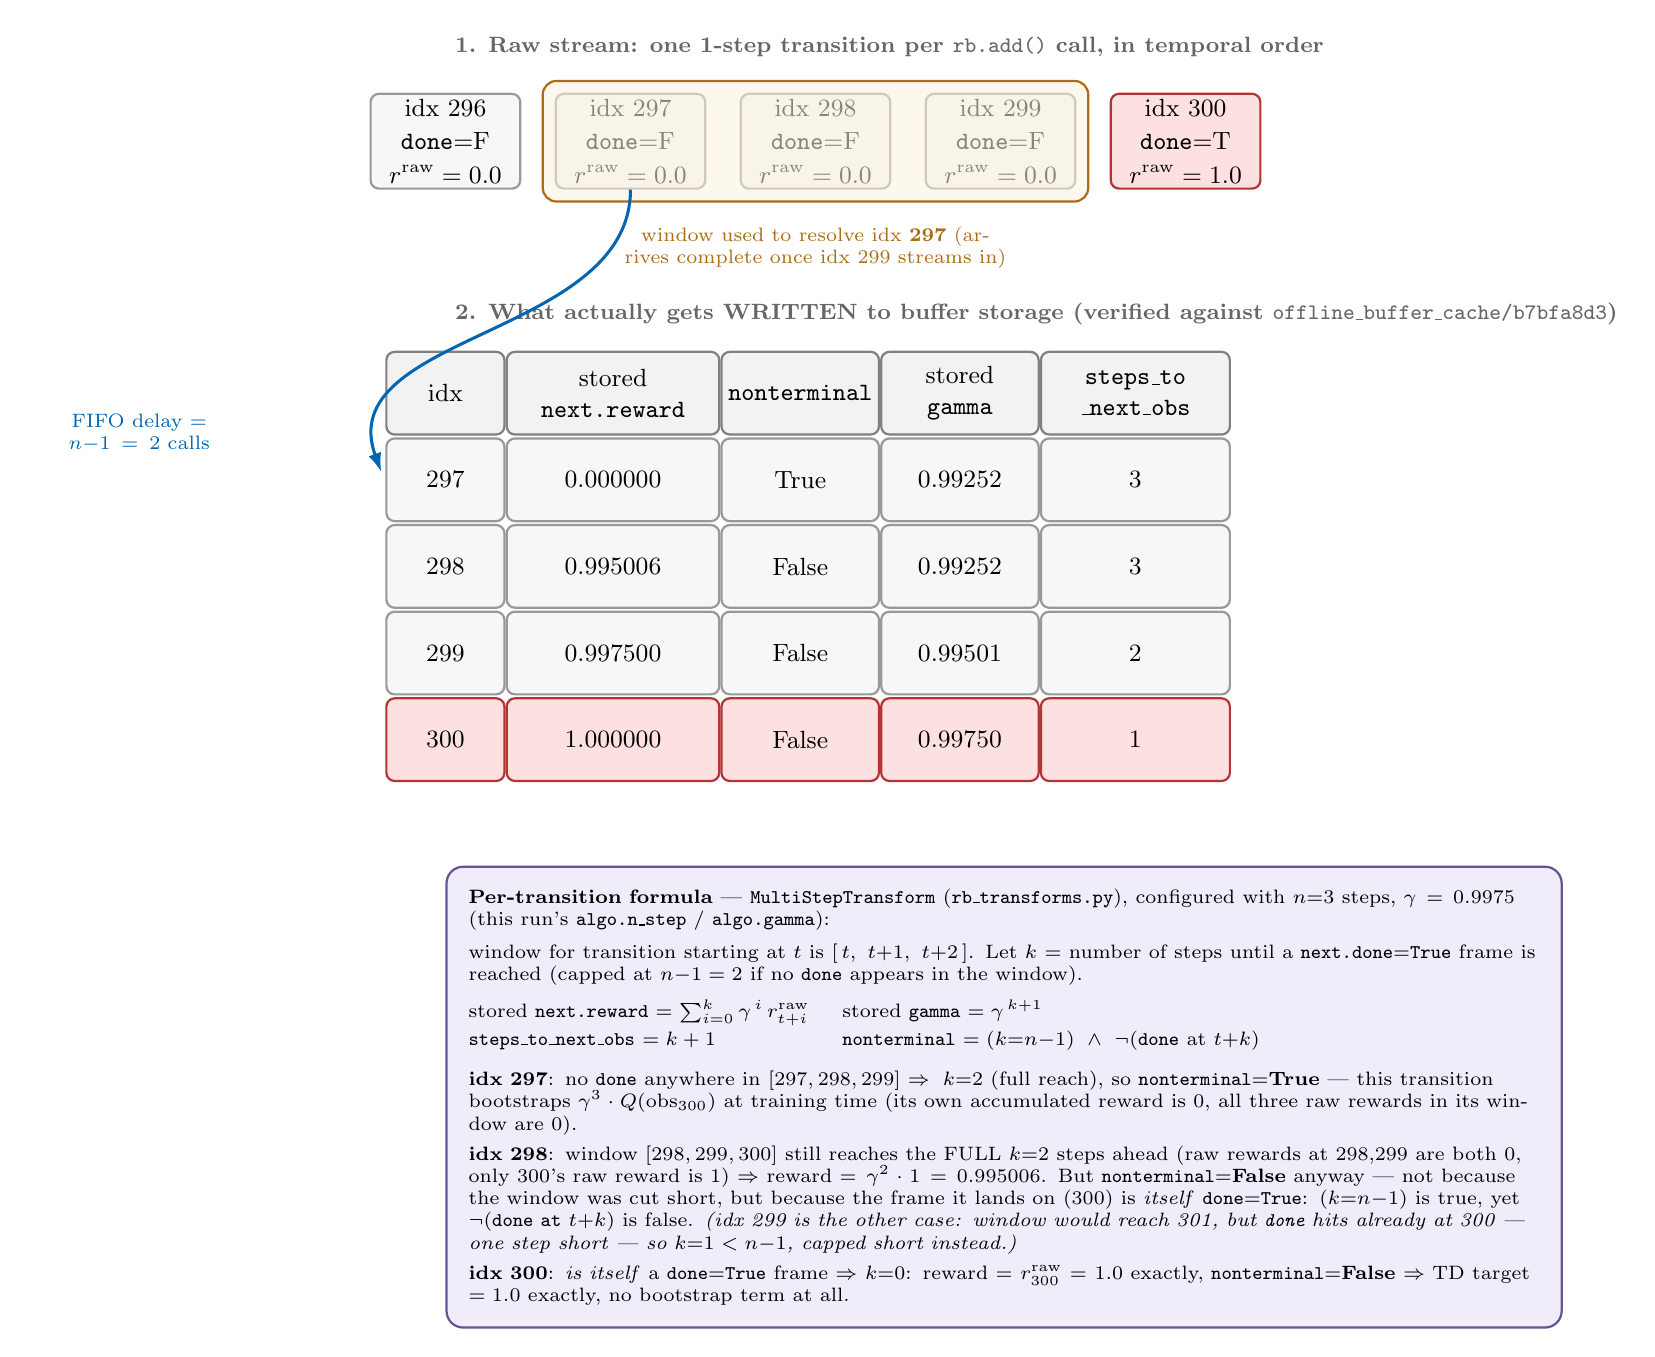
\begin{tikzpicture}[
    >={Latex[length=2.4mm,width=1.7mm]}, font=\small,
    frame/.style={draw,thick,rounded corners=3pt,align=center,minimum width=1.9cm,minimum height=1.05cm,inner sep=2pt,fill=white},
    donetrue/.style={frame,draw=doneline,fill=donefill},
    donefalse/.style={frame,draw=black!40,fill=black!3},
    hdrcell/.style={frame,fill=black!5,draw=black!50},
    writearrow/.style={->,line width=1.1pt,draw=writeline},
    lbl/.style={font=\scriptsize,align=center,text=black!70},
    hdr/.style={font=\small\bfseries,text=black!60},
]

\definecolor{bufline}{RGB}{170,108,20}   \definecolor{buffill}{RGB}{252,242,222}
\definecolor{doneline}{RGB}{178,52,52}   \definecolor{donefill}{RGB}{253,225,225}
\definecolor{writeline}{RGB}{0,102,178}
\definecolor{tgtline}{RGB}{104,84,146}   \definecolor{tgtfill}{RGB}{240,236,250}

% ---------- Section 1 title ----------
\node[hdr,anchor=west] at (0,8.4) {\footnotesize 1. Raw stream: one 1-step transition per \texttt{rb.add()} call, in temporal order};

% ---------- Row 1: raw transitions idx 296..300 (y = 7.2) ----------
\foreach \i/\idx/\done/\r in {0/296/F/0.0, 1/297/F/0.0, 2/298/F/0.0, 3/299/F/0.0, 4/300/T/1.0}{
  \pgfmathsetmacro{\x}{\i*2.35}
  \ifnum\i=4
    \node[donetrue] (f\i) at (\x,7.2) {idx \idx\\[1pt]\texttt{done}=\done\\[1pt]$r^{\text{raw}}=\r$};
  \else
    \node[donefalse] (f\i) at (\x,7.2) {idx \idx\\[1pt]\texttt{done}=\done\\[1pt]$r^{\text{raw}}=\r$};
  \fi
}

% ---------- FIFO window rectangle (idx 297,298,299) + caption BELOW it ----------
\draw[draw=bufline,thick,rounded corners=5pt,fill=buffill,fill opacity=0.55]
  ($(f1.north west)+(-0.15,0.15)$) rectangle ($(f3.south east)+(0.15,-0.15)$);
\node[lbl,text=bufline,anchor=north,align=center,text width=6.5cm] at ($(f2.south)+(0,-0.35)$)
  {window used to resolve idx \textbf{297} (arrives complete once idx 299 streams in)};

% ---------- Section 2 title (y = 5.0) ----------
\node[hdr,anchor=west] at (0,5.0) {\footnotesize 2. What actually gets WRITTEN to buffer storage (verified against \texttt{offline\_buffer\_cache/b7bfa8d3})};

% ---------- Table: header row at y=4.0, data rows below ----------
\def\tablerow#1#2#3#4#5#6#7{%
  \begin{scope}[start chain=r#1 going right, node distance=0mm, shift={(0,#7)}]
    \node[#6,minimum width=1.5cm,on chain] {#1};
    \node[#6,minimum width=2.7cm,on chain] {#2};
    \node[#6,minimum width=2.0cm,on chain] {#3};
    \node[#6,minimum width=2.0cm,on chain] {#4};
    \node[#6,minimum width=2.4cm,on chain] {#5};
  \end{scope}
}

\tablerow{idx}{stored\\\texttt{next.reward}}{\texttt{nonterminal}}{stored\\\texttt{gamma}}{\texttt{steps\_to}\\\texttt{\_next\_obs}}{hdrcell}{4.0}
\tablerow{297}{0.000000}{True}{0.99252}{3}{donefalse}{2.9}
\tablerow{298}{0.995006}{False}{0.99252}{3}{donefalse}{1.8}
\tablerow{299}{0.997500}{False}{0.99501}{2}{donefalse}{0.7}
\tablerow{300}{1.000000}{False}{0.99750}{1}{donetrue}{-0.4}

% ---------- Arrow from raw idx297 down to the written idx297 row ----------
\draw[writearrow] (f1.south) to[out=-90,in=110] ($(r297-1.west)+(-0.05,0.1)$);
\node[lbl,text=writeline,align=center,text width=2.6cm,anchor=east] at ($(r297-1.west)+(-1.7,0.6)$)
  {\scriptsize FIFO delay $=n{-}1=2$ calls};

% ---------- Formula box, clearly below the table (table bottom row at y=-0.4-0.52=-0.92) ----------
\node[draw=tgtline,thick,rounded corners=6pt,fill=tgtfill,align=left,
      font=\scriptsize,inner sep=8pt,text width=13.6cm,anchor=north west]
      at (0,-2.0) {
  \textbf{Per-transition formula} — \texttt{MultiStepTransform} (\texttt{rb\_transforms.py}), configured with $n{=}3$ steps, $\gamma=0.9975$ (this run's \texttt{algo.n\_step} / \texttt{algo.gamma}):\\[4pt]
  window for transition starting at $t$ is $[\,t,\ t{+}1,\ t{+}2\,]$. Let $k$ = number of steps until a \texttt{next.done}=\texttt{True} frame is reached (capped at $n{-}1=2$ if no \texttt{done} appears in the window).\\[4pt]
  \begin{tabular}{@{}ll@{}}
  stored \texttt{next.reward} $= \sum_{i=0}^{k} \gamma^{\,i}\, r^{\text{raw}}_{t+i}$
    & stored \texttt{gamma} $= \gamma^{\,k+1}$ \\[2pt]
  \texttt{steps\_to\_next\_obs} $= k+1$
    & \texttt{nonterminal} $= (k{=}n{-}1)\ \wedge\ \lnot(\texttt{done}\text{ at } t{+}k)$ \\
  \end{tabular}\\[6pt]
  \textbf{idx 297}: no \texttt{done} anywhere in $[297,298,299]$ $\Rightarrow k{=}2$ (full reach), so \texttt{nonterminal}=\textbf{True} — this transition bootstraps $\gamma^3\cdot Q(\text{obs}_{300})$ at training time (its own accumulated reward is 0, all three raw rewards in its window are 0).\\[3pt]
  \textbf{idx 298}: window $[298,299,300]$ still reaches the FULL $k{=}2$ steps ahead (raw rewards at 298,299 are both 0, only 300's raw reward is 1) $\Rightarrow$ reward $=\gamma^2\cdot 1=0.995006$. But \texttt{nonterminal}=\textbf{False} anyway — not because the window was cut short, but because the frame it lands on (300) is \emph{itself} \texttt{done}=\texttt{True}: $(k{=}n{-}1)$ is true, yet $\lnot(\texttt{done at }t{+}k)$ is false. \emph{(idx 299 is the other case: window would reach 301, but \texttt{done} hits already at 300 — one step short — so $k{=}1<n{-}1$, capped short instead.)}\\[3pt]
  \textbf{idx 300}: \emph{is itself} a \texttt{done}=\texttt{True} frame $\Rightarrow k{=}0$: reward $= r^{\text{raw}}_{300}=1.0$ exactly, \texttt{nonterminal}=\textbf{False} $\Rightarrow$ TD target $=1.0$ exactly, no bootstrap term at all.
};

\end{tikzpicture}
\end{document}
